\documentclass[journal=langd5,manuscript=article]{achemso}
\usepackage{lipsum}
%\usepackage[margin=1in]{geometry}
\usepackage{rotating}
\usepackage{lscape}
\usepackage[T1]{fontenc}
\usepackage[utf8]{inputenc}
\usepackage{flafter}
%\usepackage{floatflt}
\usepackage{placeins}
\usepackage{siunitx}
\usepackage{graphicx}
\graphicspath{{./figures/}}% Include figure files
%\usepackage{epstopdf}
\usepackage{dcolumn}% Align table columns on decimal point
\usepackage{appendix}
\usepackage{amsmath}
\usepackage{cases}
\usepackage{calc}
\usepackage{amssymb}
\usepackage[dvips]{color}
\usepackage{color}
\usepackage{enumitem}
\usepackage{soul}
\usepackage{indentfirst}
\usepackage{hyphenat}
\usepackage{xspace}
\usepackage{subcaption}
\usepackage{booktabs}
\usepackage{multirow}
\usepackage{tabularx}
\usepackage{xcolor}
\usepackage{lineno}
\usepackage{setspace}
\usepackage{hyperref}
\usepackage{xr-hyper}
\usepackage[nameinlink]{cleveref}
\newcommand{\tbxmulticol}[3]
    {\multicolumn{#1}
                 {>{\centering\hsize=\dimexpr#1\hsize+#1\tabcolsep+\arrayrulewidth\relax}#2}
                 {#3}}
\newcommand{\ra}[1]{\renewcommand{\arraystretch}{#1}}
%\newcommand{\cmpersec}{$\frac{\text{cm}}{\text{s}}$~}
\newcommand{\cmpersec}{cm/s~}
\newcommand{\etal}{\textit{et al.}}
\newcommand{\na}{Na\textsuperscript{+}}
\newcommand{\li}{Li\textsuperscript{+}}
\newcommand{\mg}{Mg\textsuperscript{2+}}
\newcommand{\cl}{Cl\textsuperscript{-}}
\newcommand{\mgcl}{MgCl\textsubscript{2}}
\newcommand{\nacl}{NaCl}
\newcommand{\licl}{LiCl}
\newcommand{\PM}{$\pm$~}
\newcommand{\invnm}{$\text{\si{\nm}}^{-1}$~}
\newcommand{\nmeter}{\si{\nm}~}
\renewcommand{\arraystretch}{1.8}
\newcommand{\TODO}{\hl{TODO}~}
\newcommand{\about}{$\sim$}
\newcommand{\aangstroms}{{\aa}ngstr{\"o}ms}
\newcommand{\aangstrom}{{\aa}ngstr{\"o}m}
\newcommand{\sigmaij}{$\sigma_{ij}$}
\newcommand{\epsilonij}{$\epsilon_{ij}$}
\newcommand{\db}{$\text{D}_\text{B}$}
\newcommand{\dhh}{$\text{D}_\text{hh}$}
\newcommand{\dc}{$\text{2D}_\text{C}$}
\newcommand{\Vh}{$\text{V}_\text{H}$}
\newcommand{\Vc}{$\text{V}_\text{C}$}
\newcommand{\Vl}{$\text{V}_\text{L}$}
\newcommand{\al}{$\text{A}_\text{L}$}
\newcommand{\beginsupplemental}{%
    \setcounter{table}{0}
    \renewcommand{\thetable}{S\arabic{table}}%
    \setcounter{figure}{0}
    \renewcommand{\thefigure}{S\arabic{figure}}%
}

\title{Alteration of lipid bilayer structure by \mg}
\author{Matthew Saunders}
\email{mwsaunders@usf.edu}
\affiliation{Department of Molecular Biosciences
University of South Florida, Tampa, Florida 33620}
\affiliation{Department of Physics, University of South Florida, Tampa
Florida 33620}
\author{Sagar A. Pandit}
%\email{pandit@usf.edu}
\affiliation{Department of Physics, University of South Florida, Tampa
Florida 33620}
\author{Sameer Varma}
\email{svarma@usf.edu}
\affiliation{Department of Molecular Biosciences, University of South Florida, Tampa
Florida 33620}



\date{\today}


\begin{document}
\beginsupporting
\begin{table}[h!]
    \tiny
\begin{tabularx}{\textwidth}{X|X|X|X}
\hline
\textbf{Parameter} & \textbf{Min} & \textbf{Max} & \textbf{Additional Constraint} \\
\hline
MGCH3-$\varepsilon$                   & 0.0 & 2.19239 & \\\hline
MGCH3-$\sigma$                        & 0.2 & 0.5     & \\\hline
MGCH2-$\varepsilon$                   & 0.0 & 2.13238 & \\\hline
MGCH2-$\sigma$                        & 0.2 & 0.5     & \\\hline
MGOA-$\varepsilon$                    & 0.0 & 30.0    & \\\hline
MGOA-$\sigma$                         & 0.2 & 0.5     & \\\hline
MGP-$\varepsilon$                     & 0.0 & 30.0    & \\\hline
MGP-$\sigma$                          & 0.2 & 0.5     & \\\hline
MGOM\textsuperscript{*}-$\varepsilon$ & 0.0 & 30.0    & \\\hline
MGOM\textsuperscript{*}-$\sigma$      & 0.2 & 0.5     & $\sigma_{\text{MG-OM}^*} = \min\big\{\sigma_{\text{MG-P}},\ \sigma_{\text{MG-OM}^*}\big\} $\\\hline
MGCO\textsuperscript{*}-$\varepsilon$ & 0.0 & 2.06152 & \\\hline
MGCO\textsuperscript{*}-$\sigma$      & 0.2 & 0.5     & \\\hline
MGO\textsuperscript{*}-$\varepsilon$  & 0.0 & 30.0    & \\\hline
MGO\textsuperscript{*}-$\sigma$       & 0.2 & 0.5     & \\\hline
\hline
\end{tabularx}
\caption{Parameter bounds and active constraints. $\varepsilon$ and $\sigma$ correspond to Lennard-Jones well depth and size.}
\label{tab:constrain}
\end{table}
\begin{landscape}
\centering
\begin{figure}
    \caption{Comparison between distances of \mg~atom from other atoms in clusters optimized using QM and MM.}
    \label{fig:optres}
%    \raisebox{1.2ex}{\textbf{(A)}}
%    \includegraphics[height=0.25\textheight]{figures/alloxygenconstrainedaroundpointMG6Fadded0_31_energies_nowater.eps}
%    \hspace{1em}
%    \raisebox{1.2ex}{\textbf{(B)}}
%    \includegraphics[height=0.25\textheight]{figures/alloxygenconstrainedaroundpointMG6Fadded0_31_energies.eps}
%    \hspace{1em}
%    \raisebox{1.2ex}{\textbf{(C)}}
    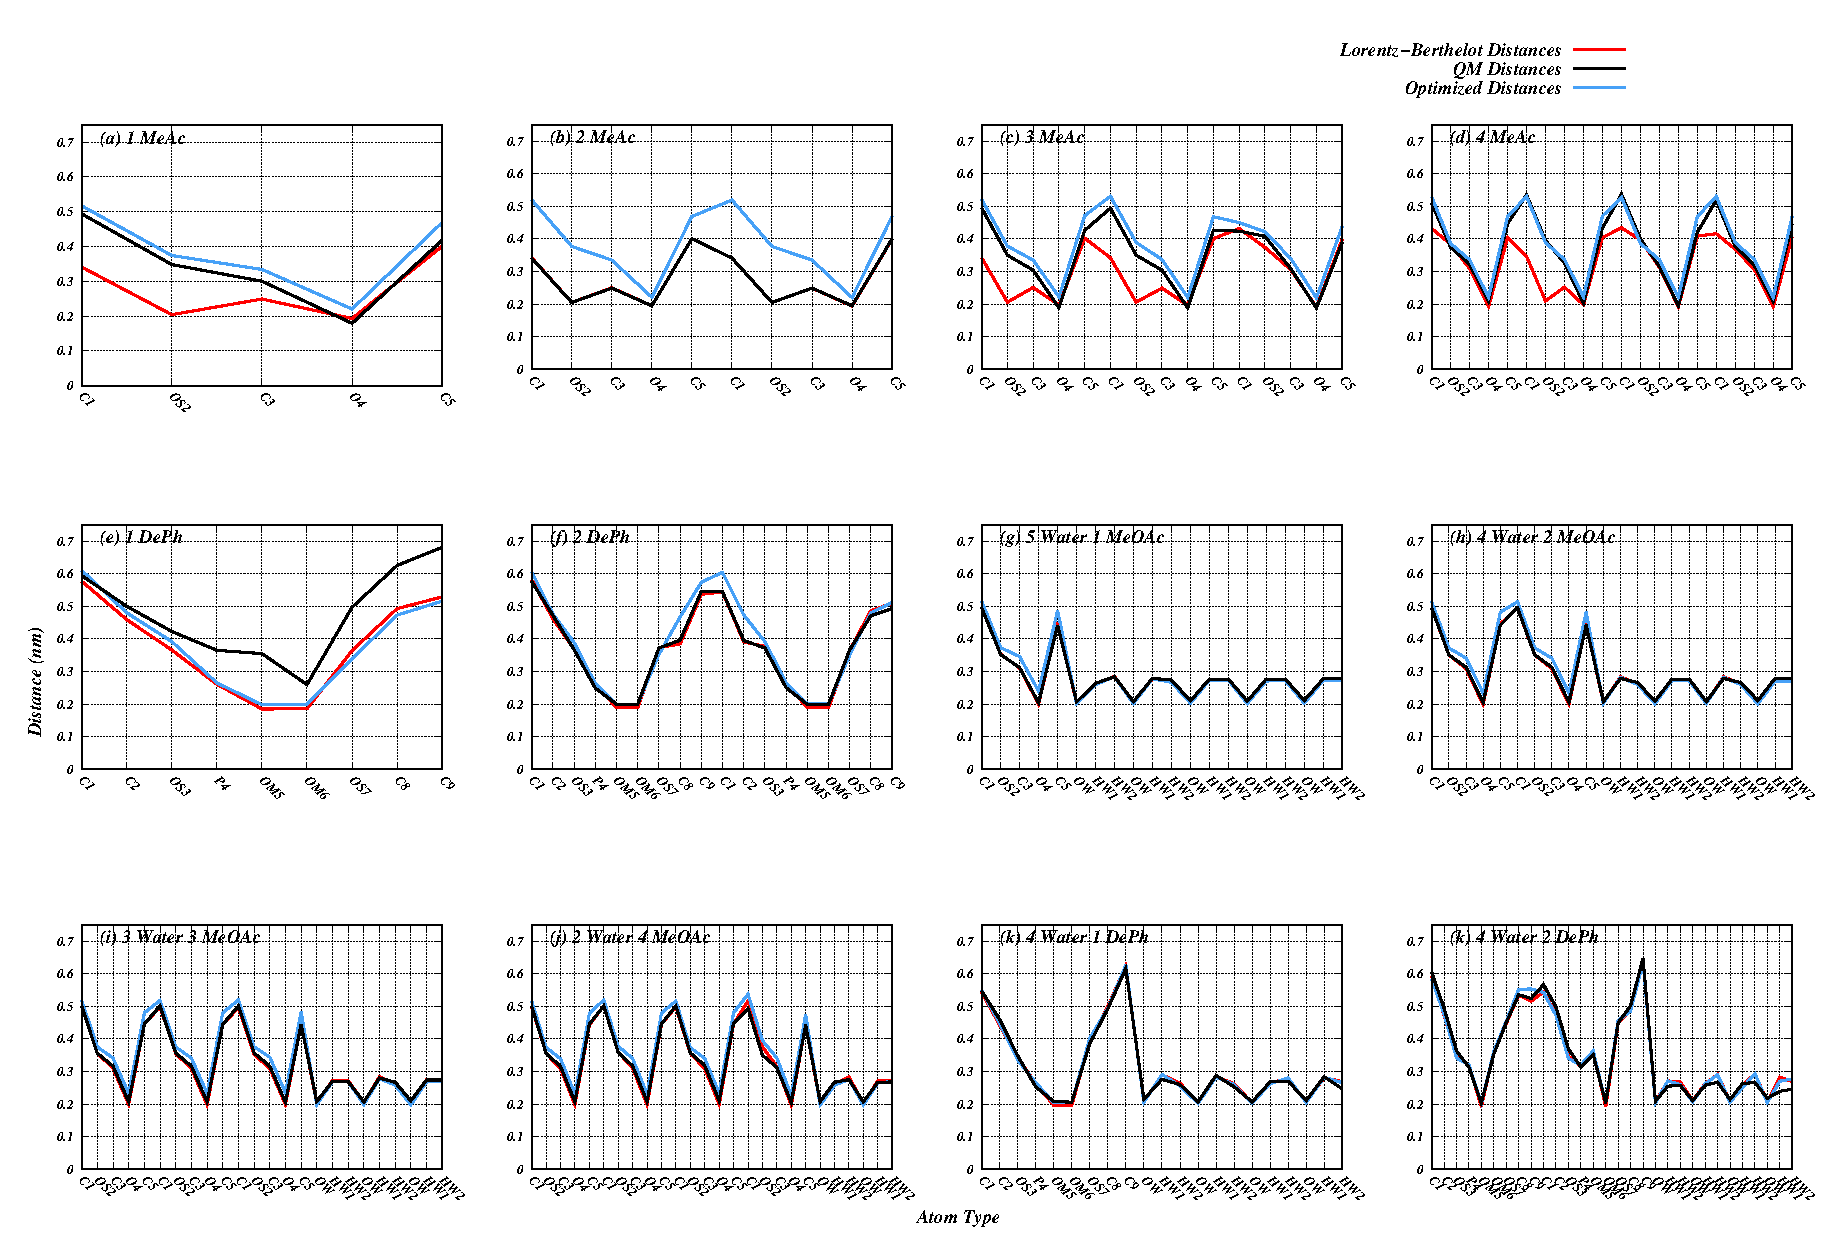
\includegraphics[height=\textheight]{figures/Figure_S1.eps}
%    \hspace{1em}
\end{figure}
\end{landscape}
%\bibliography{refs}
\end{document}
